\documentclass[UTF8]{article}
\usepackage{CTEX}
\usepackage{amsmath}
\usepackage{subcaption}
\usepackage{graphicx}
\usepackage{siunitx}
\usepackage{booktabs}
\begin{document}
    \section{研究背景与问题重述}
    \subsection{研究背景}
    随着经济的快速发展,城市机动车保有量持续上升,居民出行机不可挡。随着交通运输水平的提高,对交通运输的总需求不断增加。如今,主要城市道路日益拥挤被认为是世界上普遍的现象一个社会问题,
    它的出现使得城市的可持续发展轨迹与人民的日常生活和工作秩序发生了严重的质的变化。
    道路基础设施增长速度远不如机动车的增长速度快需求与交通供给不平衡,导致交通频繁拥堵,给城市交通形势带来了新的挑战[2]。为了缓解交通拥堵造成的经济负增长和人们生活工作秩序的混乱,
    对交通状态进行评价是非常必要的。对于城市交通管理者来说,如何快速准确地发现交通拥堵,并根据拥堵程度采取有效的对策,对于缓解交通拥堵有着重要的作用。
    交通参与者可以根据交通状态信息选择更平坦的道路线路出行可以缓解路段拥挤的压力,达到减少交通拥堵的程度。\\
    道路交叉口是车辆和行人聚集、转弯和疏散的场所,是交通的咽喉。因此,正确设计交叉口道路,合理组织、管理交叉口交通,是提高道路通行能力和保证交通安全的重要手段。
    从交通拥堵评价的相关研究来看,现有的评价方法主要集中在道路和路网的评价上,相关的评价指标主要包括交叉路口饱和度、平均停车延误、交叉口速度比、交通密度等状态指标[3]。
    由于数据采集手段的限制,无法准确采集评价模型中的一些参数。虽然一些新的探测设备已经投入市场,但由于建设成本和探测效果的影响,国内城市还没有大规模安装。\\
    \subsection{问题重述}
    以上述背景为契机,题目提供了多功能电警数据(流量和车尾时距)。为了建立一个路口交通状态的评价模型,在题目已给的数据上进行数学建模,且需要回答以下两个问题:\\
    (1)基于所提供的数据,和现有的评价指标建立一个能够评价路口交通状态的数学模型。\\
    (2)基于所提供的数据和第一问的模型,建立数学模型用于路口信号灯配时方案的调优工作。
    \section{模型假设与符号说明}
    \subsection{模型假设}
    (1)假设汽车在经过交叉路口后分别在四条道路的区间速度是均匀的;\\
    (2)假设汽车在观山东路和长岭路交叉路口通过红绿灯的速度为最大限速30码;\\
    \subsection{符号说明}
    
    \begin{table}[h] 
        \centering
        \caption{符号说明}
         
         \label{table_time}
         \resizebox{\textwidth}{!}{
         \begin{tabular}{lllllll}
         
        \toprule  
         
          指标符号 & 符号说明  & 单位 \\
               
         
        \midrule  
         
          $\mathcal{Q}$  & 某一方向的车流驶入量 & ——  \\ 
         
          $\nu$  & 平均车尾时距 &   s  \\
          \bottomrule 
         
        \end{tabular}
         }
        \end{table}
    \section{数据预处理}
    \subsection{交叉运行状态评价指标}
    根据城市道路交叉口的功能及交通特性,本文使用的交叉口评价指标包括:交通量、平均速度比、平均车尾时距。
    \subsubsection{交通量}
    交通量是指单位时间内通过道路某断面的交通流量(即单位时间通过道路某断面的车辆数目)。\\
    本文数据为3月2号到3月8号贵阳长岭路与观山东路车尾一周的时序数据,根据每抓怕一次就代表有一辆车经过的原则,可以计算出每天各路口各车道的车量总数,即日交通流,见附件。\\
    
    \begin{table}[t]
        \centering
        \caption{3月2号到3月8号各转向的车流量}
        \begin{tabular}{cccccccc}
           \hline
            转向/日期 & 2号 & 3号 & 4号 & 5号 & 6号 & 7号 & 8号 \\
           \hline
            东向西左转1	& 2935	&2942	&2949	&3091	&3003	&2289	&3168\\
           
            向西左转+直行2	&2864 &2870	&2984	&2671	&2632	&2276	&2733\\
           
            东向西直行3	&7333	&7247	&7541	&7112	&4333	&1833	&2268\\
           
            东向西直行4	&6389	&6509	&6555	&6217	&3574	&1569	&2068\\
           
            东向西右转5	&5286	&5349	&5637	&5168	&3458	&1510	&1798\\
           
            西向东左转1	&1886	&2171	&2553	&2350	&2153	&1802	&2595\\
           
            西向东左转2	&1971	&2103	&2210	&2066	&2103	&1592	&2355\\
           
            西向东左转3	&4316	&4488	&4822	&4627	&4682	&3687	&4369\\
           
            西向东直行4	&6569	&6013	&5852	&5453	&5205	&4307	&5382\\
           
            西向东东直行5	&6880	&6671	&7767	&7278	&6863	&6112	&4760\\
           
            西向东直行6	&4974	&4752	&5414	&5083	&4629	&3885	&3051\\
           
            西向东右转+直行7	&3921	&3587	&4360	&3529	&3274	&2951	&2383\\
           
            南向北左转1	&2022	&1979	&2030	&1668	&1445	&1648	&1911\\
           
            南向北左转2	&2319	&2234	&2249	&2014	&1764	&1894	&2120\\
           
            南向北左转3	&2184	&2196	&2358	&1940	&1749	&1785	&1911\\
           
            南向北直行4	&2187	&2396	&3235	&3045	&2878	&2316	&3080\\
           
            南向北直行5	&2186	&2496	&3117	&3034	&2770	&2340	&3196\\
           
            南向北直行6	&1995	&2323	&2752	&2711	&2361	&1929	&2931\\
           
            南向北直行7	&1791	&2065	&2487	&2294	&1895	&1533	&2598\\
           
            南向北右转+直行8	&1218	&1415	&1790	&1550	&1308	&1176	&1770\\
                       
            南向北右转9	&5323	&5739	&7417	&6565	&5893	&4569	&6752\\
           
            北向南左转1	&1517	&1530	&1469	&1344	&1254	&1193	&1335\\
           
            北向南左转2	&1860	&1887	&1793	&1786	&1619	&1523	&1635\\
           
            北向南左转3	&1989	&2065	&1871	&1873	&1723	&1582	&1785\\
           
            北向南左转+直行4	&6165	&6095	&6349	&5814	&5769	&5122	&6931\\
           
            北向南直行5	&7357	&7589	&7591	&7193	&7058	&6363	&8627\\
           
            北向南直行6	&7018	&7102	&7177	&6269	&6242	&5586	&7524\\
           
            北向南直行7	&899	&961	&814	&769	&684	&631	&785\\
           
            北向南右转+直行8	&1155	&1228	&1036	&1035	&873	&804	&995\\
           
            北向南右转9	&1132	&1296	&1044	&1104	&994	&833	&1045\\
           
            总计	&105641	&107298	&115223	&106653	&94188	&76640	&93861\\
           \hline
            
        \end{tabular}
    \end{table}
    由表 1可知3月4号,即星期五的车流量最高,且北向南左转+直行4、北向南直行5、
    北向南直行6、南向北右转9、东向西直行3等路线的日交通流相对较大。分别达到了6349、7591、7177、7417、7541车次。\\
    以30分钟为一个时间段,上北下南,左西右东为方向,将30个转向划分为向北驶入车辆、向西驶入车辆、向南驶入车辆、向东驶入驶入,则可以统计出7天内共336个时间段向北、向西、向南、向东这四个方向的汽车驶入量,记为$Q_ij$  ,其中$i=1,2,3,4$,代表向北、向西、向南、向东驶入,$j=1,⋯336$,代表第$j$个时间段。各方向划分,见图 1\\
    \begin{figure}[h!]
        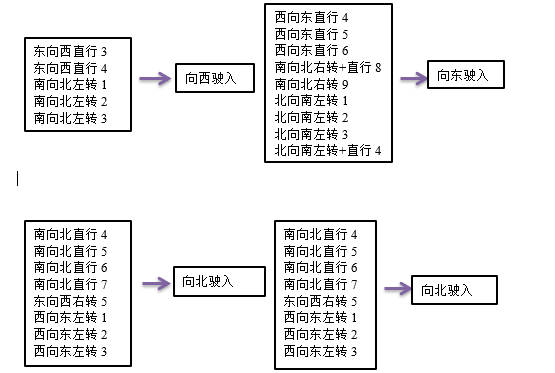
\includegraphics[width=\linewidth]{1.jpg}
        \caption{划分准则}
        \label{fig:ph1}
        
        
    \end{figure}


    
\end{document}